\section{Regime-Adaptive Risk-Aware World-Model Control}
\label{sec:ra_method}

The proposed controller retains the learned latent dynamics, force predictor,
and policy prior of TD-MPC2. Its contribution is
to couple these components through a causal, state-dependent planning
objective rather than a fixed force threshold. The policy prior proposes
candidate actions in every contact regime. A single model-predictive path
integral (MPPI) planner then changes its objective and computational budget
according to the current force state and the model's predicted transient-risk
estimate. No classical force controller, post-hoc action projection, or
evaluation-time teacher is introduced.
Figure~\ref{fig:ra_rmppi_architecture} summarizes the resulting data flow.

\begin{figure*}[t]
\centering
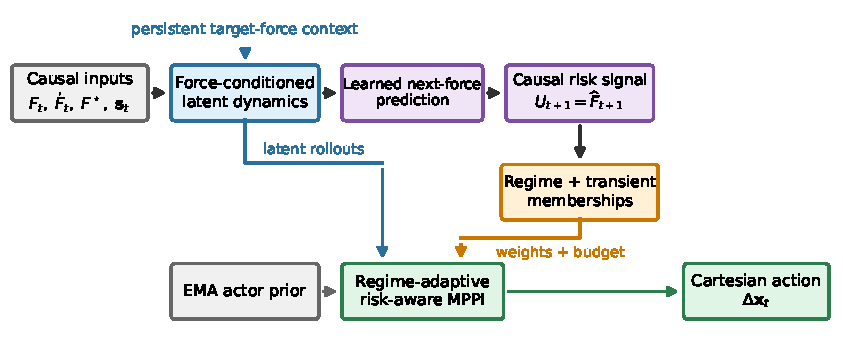
\includegraphics[width=0.96\textwidth]{figures/ra_rmppi_architecture.pdf}
\caption{Force-conditioned regime-adaptive risk-aware MPPI architecture.}
\label{fig:ra_rmppi_architecture}
\end{figure*}

Let $F_t$, $F^\star$, and $\dot F_t$ denote measured force, requested force,
and measured force rate. Unlike an observation-only target input, the requested
force is encoded by a dedicated condition branch
$\mathbf c_t=e_\theta(F^\star)$. The latent state concatenates a base state and
this condition, $\mathbf z_t=[h_\theta(\mathbf o_t);\mathbf c_t]$, and the
imagined transition is
\begin{equation}
\mathbf z_{t+1}=
\left[f_\theta(\mathbf z_t,\mathbf a_t,\mathbf c_t);\mathbf c_t\right].
\label{eq:force_conditioned_dynamics}
\end{equation}
The copied condition prevents the requested force from being diluted over a
multi-step rollout while the learned base dynamics remain action dependent.
For candidate action $\mathbf a_t$, the selected world-model risk
representation is the predicted next force
\begin{equation}
U_{t+1}=\widehat F_{t+1}.
\label{eq:ra_upper_prediction}
\end{equation}
During an $H$-step imagined rollout, this head is evaluated after every
latent transition, producing the causal transient forecast
$\widehat{\mathbf F}_{t+1:t+H}$ used by the tracking and transient costs.
This choice follows a matched development ablation against a learned
transient-envelope point prediction and a target-calibrated alternative;
neither alternative improved the prespecified outcomes.

Smooth causal memberships
\begin{equation}
\boldsymbol\pi_t=
[\pi_t^{\mathrm{acq}},\pi_t^{\mathrm{app}},
\pi_t^{\mathrm{track}},\pi_t^{\mathrm{rec}}]
\end{equation}
distinguish initial contact
acquisition, approach to the force target, stable tracking, and recovery after
contact loss. A fifth, overlapping membership $\pi_t^{\mathrm{tr}}$ measures
transient risk from $U_{t+1}$ and positive force rate. These memberships depend
only on $(F_t,F^\star,\dot F_t,U_{t+1})$ and episode-level contact history.
They replace the previous hard switch at $0.85F^\star$.

Let $r_t=\max(F_t,0)/F^\star$, let
$\sigma(x)=(1+\exp(-x))^{-1}$, and let $h_t\in\{0,1\}$ record whether
contact has occurred earlier in the episode. The unnormalized phase scores are
\begin{align}
\widetilde\pi_t^{\mathrm{acq}}
  &=(1-h_t)\sigma\!\left(10\frac{3-F_t}{F^\star}\right),\\
\widetilde\pi_t^{\mathrm{rec}}
  &=h_t\sigma\!\left(10(0.65-r_t)\right),\\
\widetilde\pi_t^{\mathrm{app}}
  &=\sigma\!\left(10(0.90-r_t)\right),\\
\widetilde\pi_t^{\mathrm{track}}
  &=\exp\!\left[-\frac{1}{2}\left(\frac{r_t-1}{0.15}\right)^2\right].
\end{align}
Normalizing these four scores gives $\boldsymbol\pi_t$. Transient membership
overlaps the phase simplex:
\begin{align}
\pi_t^{\mathrm{tr}}=1
&-\left[1-\sigma\!\left(10\frac{U_{t+1}-14.5}{0.5}\right)\right]\nonumber\\
&\quad\times\left[1-\sigma\!\left(10\left(\frac{\max(\dot F_t,0)}{80}-1\right)\right)\right].
\label{eq:transient_membership}
\end{align}
Forces are in newtons and force rate is in newtons per second. The membership
is therefore high when either the predicted next force approaches the force
limit or measured force rises rapidly.

The force thresholds in these memberships inherit the task contract in
Sec.~\ref{subsec:task}. The remaining ratios, bandwidth, sigmoid gain, and
force-rate scale are development-fixed design parameters: they create smooth,
overlapping transitions rather than learned decision boundaries. They were
held fixed before the nine-block evaluation, and no coefficient in
Eqs.~\eqref{eq:transient_membership}--\eqref{eq:adaptive_weights} was fitted on
those final blocks.

For a candidate sequence $\mathbf a_{t:t+H-1}$, the planner maximizes
\begin{align}
J_t={}&J_{\mathrm{task}}
-\lambda_c(\boldsymbol\pi_t)J_{\mathrm{contact}}
-\lambda_f(\boldsymbol\pi_t)J_{\mathrm{tracking}}\nonumber\\
&-\lambda_r(\boldsymbol\pi_t)J_{\mathrm{transient}}
-\lambda_a(\boldsymbol\pi_t)J_{\mathrm{anchor}},
\label{eq:ra_objective}
\end{align}
where $J_{\mathrm{tracking}}$ penalizes predicted force error,
$J_{\mathrm{contact}}$ penalizes predicted loss of useful contact,
$J_{\mathrm{transient}}$ penalizes predicted next force above the
soft force margin and rejects candidates at the sampled force limit, and
$J_{\mathrm{anchor}}$ regularizes search around the learned policy prior.
The four coefficients are continuous functions of the causal memberships.
Contact restoration is emphasized during acquisition and recovery, force
accuracy during approach and tracking, and transient restraint when predicted
risk or positive force rate rises.

Specifically, with
$q_t=\operatorname{clip}_{[0,1]}(\pi_t^{\mathrm{tr}}+
0.35\pi_t^{\mathrm{rec}}+0.15\pi_t^{\mathrm{acq}})$, the implemented weights
are
\begin{align}
\lambda_c &=8(\pi_t^{\mathrm{acq}}+\pi_t^{\mathrm{rec}}
                    +0.25\pi_t^{\mathrm{app}}),\\
\lambda_f &=6(0.20+0.80\pi_t^{\mathrm{track}}
                    +0.45\pi_t^{\mathrm{app}})(1-0.70\pi_t^{\mathrm{tr}}),\\
\lambda_r &=100(0.10+1.90q_t),\qquad
\lambda_a=1+1.50q_t.
\label{eq:adaptive_weights}
\end{align}

The same memberships determine the MPPI sample count, number of optimization
iterations, and proposal standard deviation. Stable tracking uses the smallest
budget. Contact acquisition and recovery use a broader proposal distribution,
whereas a high-risk transient uses more samples with a narrower distribution.
The priority is transient ($\pi_t^{\mathrm{tr}}\geq0.5$), recovery
($\pi_t^{\mathrm{rec}}\geq\max(\pi_t^{\mathrm{acq}},0.35)$), acquisition
($\pi_t^{\mathrm{acq}}\geq0.35$), approach
($\pi_t^{\mathrm{app}}>\pi_t^{\mathrm{track}}$), and then tracking.
This changes computation and exploration without changing the Cartesian action
interface. Every control step records the memberships, objective weights,
next-force risk prediction, selected budget, and issued action so that the
adaptive mechanism can be evaluated separately from task outcome.

The fixed-planner anchor uses 128 samples, 16 elites, four optimization
iterations, and maximum proposal standard deviation 0.25. The adaptive table
keeps the elite fraction at $1/8$, bounds sampling between $0.75\times$ and
$2\times$ the 128-sample anchor, and uses two to four optimization iterations.
These choices encode a monotone compute allocation across nominal tracking,
contact restoration, and transient risk; the matched component ablation tests
the allocation as a whole rather than selecting its entries on final outcomes.

\begin{table}[t]
\centering
\caption{Regime-dependent MPPI budget.}
\label{tab:adaptive_budget}
\small
\begin{tabular}{lrrrr}
\toprule
Regime & Samples & Elites & Iterations & Max. std. \\
\midrule
Transient  & 256 & 32 & 4 & 0.10 \\
Recovery   & 160 & 20 & 3 & 0.20 \\
Acquisition& 160 & 20 & 3 & 0.20 \\
Approach   & 128 & 16 & 3 & 0.16 \\
Tracking   &  96 & 12 & 2 & 0.12 \\
\bottomrule
\end{tabular}
\end{table}

The component study compares this complete formulation with fixed-objective,
adaptive-objective-only, and adaptive-compute-only variants before the
factor-separated evaluation.
